\documentclass{article}
\usepackage{amsmath}
\usepackage{titlesec}
\usepackage{graphicx}
\usepackage[margin=1in]{geometry}

\titleformat{\section}
  {\normalfont\small\bfseries} % Format: font style, size, and weight
  {\thesection}{1em} % Label format and spacing
  {}
\titleformat{\subsection}
  {\normalfont\small\bfseries} % Format: font style, size, and weight
  {\thesection}{1em} % Label format and spacing
  {}
\titleformat{\subsubsection}
  {\normalfont\small\bfseries} % Format: font style, size, and weight
  {\thesection}{1em} % Label format and spacing
  {}

\begin{document}
\small
\subsection{Relationship between Flow Rate and Delta Pressure}
Given the Bernoulli equation:
\begin{equation}
P_1 + \frac{1}{2} \rho v_1^2 + \rho gh_1 = P_2 + \frac{1}{2} \rho v_2^2 + \rho gh_2
\end{equation}

and the continuity equation for an incompressible fluid:
\begin{align}
    A_1 v_1 &= A_2 v_2 \\
    Q_1 &= Q_2
\end{align}

we can combine these equations to derive the relationship between the pressure difference and the flow rate.
\begin{equation}
\Delta P = \frac{1}{2} \rho \left( v_2^2 - v_1^2 \right)
\end{equation}
\begin{equation}
Q = A_1 A_2\sqrt{\frac{2 \Delta P}{\rho \left( A_1^2 - A_2^2 \right)}}
\end{equation}

\subsection{Assumptions for the Application of the Bernoulli Equation}

The Bernoulli equation is derived under the assumption of ideal fluid. Thus, the key assumptions include:

\begin{enumerate}
    \item \textbf{Stationary flow}
    \item \textbf{Along a Streamline}
    \item \textbf{Incompressible fluid}
    \item \textbf{Inviscid fluid}
    \item \textbf{Non-conductive fluid}
    
\end{enumerate}

\subsection{Design Restrictions on the Venturi Nozzle Due to Bernoulli Equation Assumptions}

The design of a Venturi nozzle must consider the following restrictions due to the assumptions required for the application of the Bernoulli equation:

\begin{enumerate}
    \item \textbf{Incompressible Flow}: Ensure that the fluid is a liquid or a gas at low speeds where density changes are negligible. For gases, the Mach number should be less than 0.3.

    \item \textbf{Steady Flow}: Design the system to operate under steady-state conditions. Avoid transient conditions such as startup or shutdown phases.

    \item \textbf{Non-viscous Flow}: Minimize the effects of viscosity by ensuring smooth surfaces and streamlined flow paths within the Venturi nozzle. Use fluids with low viscosity or operate at high Reynolds numbers.

    \item \textbf{Along a Streamline}: Ensure that measurements and calculations are taken along the same streamline. Design the Venturi nozzle to have a well-defined and predictable flow path.

    \item \textbf{No Heat Transfer}: Insulate the Venturi nozzle to minimize heat transfer. Ensure that the temperature of the fluid remains constant throughout the nozzle.
    
\end{enumerate}

\subsection{Considerations for Using a Venturi Nozzle in a Heat Exchanger}

Given the previously reported assumptions of the Bernoulli equation, since the fluid is non-conductive, the Venturi nozzle cannot be used in a heat exchanger.


\section{Task 1.7: Asymptotic Suction Boundary Layer}

\subsection{Assumptions, Initial Conditions, and Boundary Conditions}

\section*{Assumptions:}
\begin{itemize}
    \item \textbf{Flat plate parallel to the flow:} The flow is two-dimensional and the plate is infinite in the \(x\) direction.
    \item \textbf{\(\frac{d}{dx} \ll \frac{d}{dy}\), \(\frac{d^2}{dx^2} \ll \frac{d^2}{dy^2}\):} Rate of change across the boundary layer is much greater than the rate of change in the flow direction.
    \item \textbf{Thin boundary layer:} \(u \gg v\)
    \item \textbf{No streamwise pressure gradient \(\frac{dp}{dx}\):} The flow is time-independent.
\end{itemize}

\section*{Initial Conditions:}
\begin{itemize}
    \item \textbf{At \(t = 0\):} The velocity field is established and steady.
\end{itemize}

\section*{Boundary Conditions:}
\begin{itemize}
    \item \textbf{At the wall \((y = 0)\):} \(u = 0\), \(v = -V_w\) (steady suction velocity).
    \item \textbf{Far from the wall \((y \rightarrow \infty)\):} \(u = U_\infty\), \(v = 0\) (free-stream conditions).
\end{itemize}

\subsection{Simplified Continuity and Navier–Stokes Equations on a 2D domain}

\section*{Continuity Equation:}
\[
\frac{\partial u}{\partial x} + \frac{\partial v}{\partial y} = 0
\]

\section*{Navier–Stokes Equations:}
\begin{align*}
    \text{x-momentum:} & \quad u \frac{\partial u}{\partial x} + v \frac{\partial u}{\partial y} = -\frac{1}{\rho} \frac{\partial p}{\partial x} + \nu (\frac{\partial^2 v}{\partial x^2}+\frac{\partial^2 v}{\partial y^2}) \\
    \text{y-momentum:} & \quad u \frac{\partial v}{\partial x} + v \frac{\partial v}{\partial y} = -\frac{1}{\rho} \frac{\partial p}{\partial y} + \nu (\frac{\partial^2 v}{\partial x^2}+\frac{\partial^2 v}{\partial y^2})
\end{align*}

Given the assumptions, the equations simplify to the so called Prandtl's boundary layer equations:
\[
\frac{\partial u}{\partial x} + \frac{\partial v}{\partial y} = 0
\]
\[
u \frac{\partial u}{\partial x} + v \frac{\partial u}{\partial y} = \nu \frac{\partial^2 u}{\partial y^2}
\]
\[
\frac{\partial p}{\partial y} = 0
\]

\subsection{Solution of Simplified PDEs}
We can solve the simplified PDEs, as Blasius did with the Similarity Ansatz, to obtain ODEs.
The system of equations becomes:
\[
\begin{cases}
f''' + 0.5 f f'' = 0 \\
f(0) = 0 \\
f'(0) = 0 \\
f'(\infty) = 1
\end{cases}
\]

We can solve the Blasius equation numerically to obtain the velocity profile. We give as u''(0)=1.5399 from the link in the \cite{NumericalMethods} citation.
Below is the solution of the Blasius equation, obtained through a python:
\begin{figure}[h]
    \centering
    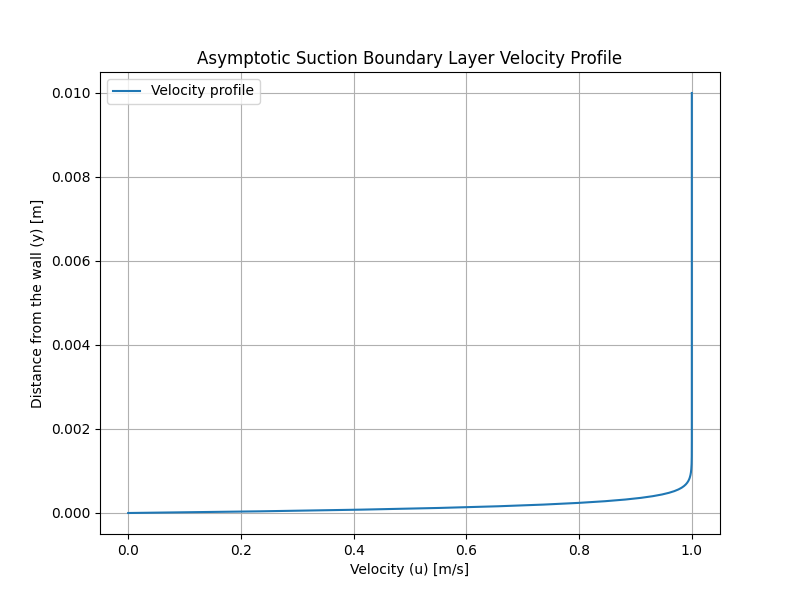
\includegraphics[width=0.8\textwidth]{output_plot.png}
    \caption{Numerical solution of the Blasius equation showing the velocity profile.}
    \label{fig:blasius_solution}
\end{figure}

In addition, we have implemented in our script the calculation of the friction coefficient and the displacement thickness, which result in:
\textbf{Results:}
\begin{itemize}
    \item \textbf{Wall Shear Stress (\(\tau_{\text{wall}}\)):} 1.5399
    \item \textbf{Friction Coefficient (\(c_f\)):} 3.0798
    \item \textbf{Pressure Coefficient (\(c_p\)):} 0.0
\end{itemize}

\subsection{Calculation of the boundary layer displacement thickness}
\section*{Boundary Layer Displacement Thickness Calculation}
The boundary layer displacement thickness (\(\delta^*\)) can be calculated using the following formula:
\[
\delta^* = \frac{1.7208 \cdot x}{\sqrt{Re_x}} = 1.7208
\]

The displacement thickness represents the distance by which the outer potential flow is displaced due to the boundary layer. It accounts for the reduction in flow rate caused by the presence of the boundary layer.

In this setup, \(\delta^*\) depends on the free-stream velocity (\(U_\infty\)), the kinematic viscosity (\(\nu\)), and the distance from the leading edge (\(x\)). As \(U_\infty\) increases, \(\delta^*\) decreases, indicating a thinner boundary layer. Conversely, as \(\nu\) or \(x\) increases, \(\delta^*\) increases, indicating a thicker boundary layer.
\subsection{Applications of the Blasius Equation}
The Blasius equation finds applications in various engineering problems where boundary layer theory is relevant. One notable example is the flow over a long train, where the flow is parallel to the length of the train and the length is significantly greater than the width. 


\begin{thebibliography}{9}

\bibitem{NumericalMethods}
  \textit{Numerical and analytical solutions of new Blasius equation for turbulent flow},
  Mizanur Rahman, Shahansha Khan, M Ali Akbar.
\end{thebibliography}
\end{document}
